% Held-out session of Study 2, in two parts for content.tex:
%   Part 1 replaces the text under \subsection{Held-Out Session} \label{sec:feas-s2-holdout}
%   Part 2 replaces the text under \subsection{Held-Out Session} \label{sec:results-s2-holdout}
%   Part 3 (optional) is a replacement for the first Study 2 bullet in \section{Limitations}
% Requires: booktabs, pgfplots (compat=1.18). No siunitx.
% Numbers: python3 scripts/analyse_privacy_switch.py study/privacy_switch_study2_holdout.csv --coords
%          venv/bin/python3 scripts/replay_privacy_switch.py study/privacy_switch_study2_holdout.csv
%          (and with --radar-module pointing at the Study 2 version of radar_ld2450.py)
% Room measurements (door frame, threshold distance) were taken by tape and are approximate.

% ======================================================================
% Part 1 - method
% ======================================================================

A second session was run on 13 September 2026, after the exit condition of
section~\ref{sec:results-s2-exit} had been added to the production logic. Its
50 trials were presented in randomised order in one continuous run of
27 minutes: 15 direct entries, 15 fast entries, 10 passes and 10 peeks
(table~\ref{tab:feas-s2-scripts}). The exit condition was active
(\texttt{EXIT\_SPEED\_MMS} = 500) and was recorded with every trial; the entry
and exit logic, the classification windows and the 15\,s stay were otherwise
those of the main session.

The session differs from the main session in four respects.

\begin{itemize}
  \item \textbf{Room.} It took place in a different room with different
  furniture. The door frame was about 0.8\,m wide and the threshold about
  4.3\,m from the sensor. The room zone spanned $x$ from $-1.63$ to 1.65\,m
  and $y$ from 0.11 to 4.31\,m. Its left and near edges were kept from the
  main session after checking in the web application that they matched the
  new room; its right and far edges were redrawn. The door zone spanned $x$
  from $-1.63$ to $-0.21$\,m and $y$ from 4.32 to 4.98\,m, so it was
  0.66\,m deep against 1.12\,m in the main session. Its left edge coincides
  with the room zone's, which is where the web application places a new door
  zone.
  \item \textbf{A seated person.} A second person sat still at the desk
  throughout, 0.66\,m in front of the sensor, in the place of a user. Before
  the first trial, 30\,s were recorded with only that person in view: the
  radar reported them in all 300 frames and never reported a second target,
  and every report lay within 476\,mm of their median position. The
  conversation partner was still registered by the harness rather than by
  that person speaking.
  \item \textbf{The same mover.} The movement scripts were again performed by
  the author. The session therefore changes the room and adds a seated
  person, but does not change the mover.
  \item \textbf{Manual return to speech.} Since the main session, the
  assistant no longer returns to speech on its own. When the radar judges the
  room clear again it signals this, and speech resumes only when the user
  asks for it (section~\ref{sec:sdi-switch}). The harness resumed speech
  between trials in the user's place, and the moment the room was judged
  clear was classified exactly as the return to speech had been: correct
  after the cue to leave, premature before it, missed if it did not occur
  within 60\,s.
\end{itemize}

The reply was synthesised once, with the voice of the main session, and
played from file in every trial; the file was verified to be identical across
all 50 trials. Playback therefore began within 6\,ms of the harness requesting
it, against a median 0.24\,s for live synthesis in the main session. One pass
was discarded by the operator with the note that nothing had been tracked and
was run again; its log was kept and is reported separately in
section~\ref{sec:results-s2-holdout}.

The session tests the exit condition on trials it was not derived from. It
does not separate the effect of the room from that of the seated person or of
the shallower door zone, since all three changed together.

% ======================================================================
% Part 2 - results
% ======================================================================

Table~\ref{tab:ps-holdout-outcomes} summarises the 50 trials by script and
table~\ref{tab:ps-holdout-compare} sets them against the main session.

\begin{table}[htb]
  \centering
  \caption{Outcome per scripted behaviour in the held-out session.
  \emph{Lowered} counts trials in which the voice was lowered at any point.}
  \label{tab:ps-holdout-outcomes}
  \begin{tabular}{llrlrr}
    \toprule
    Script & Behaviour & $n$ & Expected & Switched & Lowered \\
    \midrule
    A & Direct entry, normal pace   & 15 & switch      & 12 & 13 \\
    F & Fast entry                  & 15 & switch      & 11 &  9 \\
    D & Peek, stop in the doorway   & 10 & lower only  &  0 & 10 \\
    B & Pass close to the open door & 10 & no reaction &  0 &  0 \\
    \bottomrule
  \end{tabular}
\end{table}

\begin{table}[htb]
  \centering
  \small
  \caption{Main session and held-out session. Proportions with exact
  Clopper--Pearson 95\,\% intervals, durations as median [IQR]. In the main
  session the exit moment is the return to speech; in the held-out session it
  is the moment the room was judged clear.}
  \label{tab:ps-holdout-compare}
  \begin{tabular}{lll}
    \toprule
    & Main session & Held-out session \\
    \midrule
    Entries detected      & 53/55 (96.4\,\%; 87.5--99.6) & 23/30 (76.7\,\%; 57.7--90.1) \\
    \quad direct (A)      & 30/30 (100\,\%; 88.4--100)   & 12/15 (80.0\,\%; 51.9--95.7) \\
    \quad fast (F)        & 23/25 (92.0\,\%; 74.0--99.0) & 11/15 (73.3\,\%; 44.9--92.2) \\
    False switches        & 0/38 (0--9.3\,\%)            & 0/20 (0--16.8\,\%) \\
    \addlinespace
    Peeks lowered         & 18/18 (81.5--100\,\%)        & 10/10 (69.2--100\,\%) \\
    Passes lowered        & 9/20 (45.0\,\%; 23.1--68.5)  & 0/10 (0--30.8\,\%) \\
    \addlinespace
    Exit: correct         & 44/53 (83.0\,\%; 70.2--91.9) & 22/23 (95.7\,\%; 78.1--99.9) \\
    Exit: premature       & 8/53 (15.1\,\%; 6.7--27.6)   & 0/23 (0--14.8\,\%) \\
    Exit: missed          & 1/53 (1.9\,\%; 0.0--10.1)    & 1/23 (4.3\,\%; 0.1--21.9) \\
    \addlinespace
    Room-edge crossing $\to$ switch (s) & 0.163 [0.101, 0.179] & 0.125 [0.103, 0.159] \\
    Ground speed, fast entries (m/s)    & 1.37 [1.20, 1.44]    & 1.80 [1.66, 2.29] \\
    Door zone depth (m)                 & 1.12                 & 0.66 \\
    \bottomrule
  \end{tabular}
\end{table}

\subsubsection{Switch Decisions}

The assistant switched to the chat in 23 of 30 entries (76.7\,\%; CI
57.7--90.1\,\%), against 53 of 55 in the main session, and in none of the
20 passes and peeks (CI 0--16.8\,\%). The misses were spread over both entry
scripts: 3 of 15 direct entries and 4 of 15 fast entries. Of the 23 detected
entries, 21 were decided at the door zone and 2 by the near-door rule. The
switch followed the radar-estimated crossing of the room-zone edge by a median
0.125\,s (IQR 0.103--0.159\,s), and the voice was lowered before the switch in
21 of the 23, a median 0.51\,s (IQR 0.40--0.90\,s) beforehand.

The misses differ from the detected entries in where the radar first reported
the mover (figure~\ref{fig:ps-holdout-plan}). In 21 of the 23 detected
entries, someone other than the seated person was reported in the door zone
before the switch. In 6 of the 7 misses nobody was: in five of them the mover
was not reported beyond the door zone either, and in all six the mover was
first reported inside the room, 0.85--1.93\,m from the door zone and so beyond
the 0.8\,m near-door radius. In the seventh (trial~30), the mover's reported
path ran just beside the door zone: level with it, the reports lay at $x$
between $-0.18$ and 0.06\,m, against a door-zone edge at $-0.21$\,m. The
mover therefore reached the room from outside both zones, which by design is
not an entry. A second target reported in the door zone at the same moment
lowered the voice and was then closed as a peek.

\begin{figure}[htb]
  \centering
  \definecolor{hitc}{HTML}{2A78D6}
  \definecolor{missc}{HTML}{EB6834}
  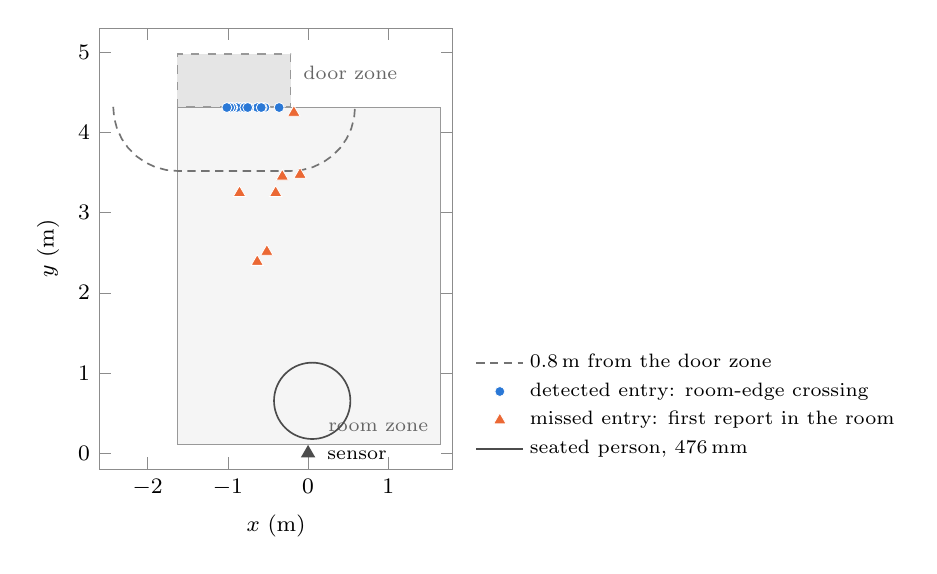
\begin{tikzpicture}
    \begin{axis}[
      axis equal image,
      width=0.5\textwidth, height=0.8\textwidth,
      xmin=-2.6, xmax=1.8, ymin=-0.2, ymax=5.3,
      xtick={-2,-1,0,1}, ytick={0,1,2,3,4,5},
      xlabel={$x$ (m)}, ylabel={$y$ (m)},
      tick label style={font=\footnotesize},
      label style={font=\footnotesize},
      axis line style={draw=black!45}, tick style={draw=black!45},
      legend style={at={(1.04,0)}, anchor=south west, font=\scriptsize,
                    draw=none, cells={anchor=west}},
    ]
      \draw[black!40, fill=black!4] (axis cs:-1.630,0.107) rectangle (axis cs:1.646,4.311);
      \draw[black!40, dashed, fill=black!10] (axis cs:-1.630,4.320) rectangle (axis cs:-0.214,4.979);
      \node[font=\scriptsize, black!60, anchor=south east] at (axis cs:1.62,0.15) {room zone};
      \node[font=\scriptsize, black!60, anchor=west] at (axis cs:-0.18,4.75) {door zone};
      \addplot[black!55, densely dashed, line width=0.6pt]
        coordinates {(-2.430,4.320) (-2.418,4.181) (-2.382,4.046) (-2.323,3.920) (-2.243,3.806)
                     (-2.144,3.707) (-2.030,3.627) (-1.904,3.568) (-1.769,3.532) (-1.630,3.520)
                     (-0.214,3.520) (-0.075,3.532) (0.060,3.568) (0.186,3.627) (0.300,3.707)
                     (0.399,3.806) (0.479,3.920) (0.538,4.046) (0.574,4.181) (0.586,4.320)};
      \addlegendentry{0.8\,m from the door zone}
      \addplot[only marks, mark=*, mark size=1.8pt,
               mark options={fill=hitc, draw=white, line width=0.3pt}, hitc]
        coordinates {(-0.974,4.311) (-0.578,4.311) (-0.971,4.311) (-0.538,4.311) (-0.849,4.311)
                     (-0.807,4.311) (-0.609,4.311) (-0.857,4.311) (-0.956,4.311) (-0.632,4.311)
                     (-0.892,4.311) (-0.939,4.311) (-0.738,4.311) (-0.949,4.311) (-0.573,4.311)
                     (-0.789,4.311) (-0.977,4.311) (-0.584,4.311) (-0.361,4.311) (-0.753,4.311)
                     (-1.013,4.311)};
      \addlegendentry{detected entry: room-edge crossing}
      \addplot[only marks, mark=triangle*, mark size=2.6pt,
               mark options={fill=missc, draw=white, line width=0.3pt}, missc]
        coordinates {(-0.634,2.387) (-0.404,3.247) (-0.855,3.246) (-0.177,4.247)
                     (-0.514,2.513) (-0.321,3.452) (-0.100,3.474)};
      \addlegendentry{missed entry: first report in the room}
      \addplot[black!70, line width=0.6pt, domain=0:360, samples=73]
        ({0.0515 + 0.476*cos(x)}, {0.6535 + 0.476*sin(x)});
      \addlegendentry{seated person, 476\,mm}
      \addplot[only marks, mark=triangle*, mark size=2.6pt, black!70, forget plot] coordinates {(0,0)};
      \node[font=\scriptsize, anchor=west] at (axis cs:0.12,-0.02) {sensor};
    \end{axis}
  \end{tikzpicture}
  \caption{Held-out session in the sensor's coordinates. Blue: where the 21
  entries decided at the door zone crossed the room-zone edge. Orange: where
  the mover was first reported inside the room in the seven missed entries;
  six lie beyond 0.8\,m from the door zone, the radius within which a newly
  acquired track can still count as an entry, and the seventh (trial~30) was
  reached from beside the door zone. The circle marks the seated person's
  baseline position and the spread of its reports.}
  \label{fig:ps-holdout-plan}
\end{figure}

What kept the radar from reporting the mover at the doorway in these trials
cannot be determined from the session. The seated person was reported in every
frame of five of the seven misses, and likewise in 20 of the 23 detected
entries, so their presence does not by itself distinguish the misses. The door zone was shallower
than in the main session (0.66 against 1.12\,m) and the fast entries were faster
(median ground speed 1.80\,m/s, IQR 1.66--2.29\,m/s, against 1.37\,m/s), both of
which leave fewer frames in which a newly acquired track can be seen in the
door zone. The room, the seated person and the door zone changed together,
so their contributions cannot be separated.

\subsubsection{Behaviour at the Door}

Every peek lowered the voice, and none switched the output (10 of 10; CI
69.2--100\,\%). The voice stayed lowered for a median 9.4\,s (IQR
9.2--9.7\,s). Peeks reached 0.50--0.66\,m past the door zone's outer edge,
which in this door zone is nearly its full depth. No pass lowered the voice
(0 of 10; CI 0--30.8\,\%) and none switched. The passes stayed further from
the door zone than in the main session: their closest approach was a median
0.44\,m (range 0.19--1.54\,m), whereas in the main session every pass came
within 0.26\,m of its edge. The absence of lowered passes is therefore not
evidence that the margin problem of section~\ref{sec:results-s2-door} has been
resolved. In the discarded pass, the radar reported the seated person in all
150 frames and nobody else at any point.

\subsubsection{Exits and the Exit Condition}

The room was judged clear correctly, after the mover had left, in 22 of the
23 detected entries (95.7\,\%; CI 78.1--99.9\,\%), prematurely in none (CI
0--14.8\,\%), and not at all in one (4.3\,\%; CI 0.1--21.9\,\%). In that one
(trial~22) the mover was not reported in the door zone on the way out. After a
correct exit, the room was judged clear a median 2.03\,s (IQR 1.91--2.19\,s)
after the mover's track crossed back out of the room zone. The one long delay,
32.6\,s in trial~35, came from a motionless target that remained in the door
zone for 31.3\,s after the mover had left. Within 0.5\,s of the crossing,
every genuine exit reached a reported radial velocity of at least
960\,mm/s (median 1190\,mm/s), well above the 500\,mm/s the exit condition
requires.

Replaying the session's radar frames offline reproduced the observed outcome
of all 50 trials, both through the logic that ran and through the logic of the
main session without the exit condition. No phantom exit of the kind that
produced the premature returns in the main session occurred in this session,
so the condition had nothing to prevent: it did not reject a genuine exit, but
the session does not show that it removes premature exits on new trials.

\subsubsection{A Seated Person and a Second Person Moving}

The seated person was reported in 94.3\,\% of all trial frames (11\,001 of
11\,662) and in every frame of 41 of the 50 trials. In frames in which nobody
else was reported, they were reported in 98.3\,\% (2\,586 of 2\,632); in
frames with another target, in 93.2\,\% (8\,415 of 9\,030). The losses were
concentrated in three trials: the seated person was not reported at all in the
180 frames of one peek (trial~9), and in only 52 of 201 and 48 of 238 frames of
two fast entries (trials~8 and~31). While the mover stood inside after a
detected entry, both people were reported in 86.6\,\% of frames, only the
seated person in 8.6\,\% and only the mover in 4.9\,\%; the mover stood a median
2.04\,m (IQR 1.89--2.22\,m) from the seated person. No entry was decided at
the seated person's position. Frame shares are given without intervals,
because consecutive frames are not independent observations.

% ======================================================================
% Part 3 (optional) - replacement for the first Study 2 bullet in Limitations
% ======================================================================

%  \item All trials were performed by a single mover (the author), who knew the
%  system and the protocol. The main session ran in one room with one door and
%  one sensor placement; the held-out session of
%  section~\ref{sec:results-s2-holdout} changed the room, added a seated person
%  and used a shallower door zone, all at once, and kept the mover. Visitors who
%  hesitate, turn back in the doorway or enter side by side were not tested.
